\documentclass[]{upb_cs_thesis} % include german inside brackets for a German thesis

% load your own packages and user-defined commands
\usepackage{amsmath, amssymb, amsfonts}% mathematical symbols and the like
\usepackage{amsthm}% definitions, theorems, etc.
\usepackage[colorinlistoftodos]{todonotes}% marking open todos in text/on margins
\usepackage{subfig}% multi-part figures with separate captions per part
\usepackage{url}% render URLs correctly and make them clickable through the hyperref package
\usepackage{longtable}% tables that span multiple pages
\usepackage{booktabs}% tables that actually look good
\usepackage[nolist]{acronym}% consistently use acronyms
\usepackage[backend=biber]{biblatex}
\addbibresource{literature.bib}
\usepackage{pgfgantt}
\usepackage{float}
\usepackage{listings}
\usepackage{graphicx}
\usepackage[export]{adjustbox}
\usepackage{xcolor}

\colorlet{punct}{red!60!black}
\definecolor{background}{HTML}{EEEEEE}
\definecolor{delim}{RGB}{20,105,176}
\colorlet{numb}{magenta!60!black}

\lstdefinelanguage{json}{
	basicstyle=\normalfont\ttfamily,
	numbers=left,
	numberstyle=\scriptsize,
	stepnumber=1,
	numbersep=8pt,
	showstringspaces=false,
	breaklines=true,
	frame=lines,
	backgroundcolor=\color{background},
	literate=
	*{0}{{{\color{numb}0}}}{1}
	{1}{{{\color{numb}1}}}{1}
	{2}{{{\color{numb}2}}}{1}
	{3}{{{\color{numb}3}}}{1}
	{4}{{{\color{numb}4}}}{1}
	{5}{{{\color{numb}5}}}{1}
	{6}{{{\color{numb}6}}}{1}
	{7}{{{\color{numb}7}}}{1}
	{8}{{{\color{numb}8}}}{1}
	{9}{{{\color{numb}9}}}{1}
	{:}{{{\color{punct}{:}}}}{1}
	{,}{{{\color{punct}{,}}}}{1}
	{\{}{{{\color{delim}{\{}}}}{1}
	{\}}{{{\color{delim}{\}}}}}{1}
	{[}{{{\color{delim}{[}}}}{1}
	{]}{{{\color{delim}{]}}}}{1},
}
\lstset{
	basicstyle=\ttfamily,
	frame=single
}
\usepackage{tikz}
\usetikzlibrary{intersections}
%%%%%%%%%
% Some commands for setting up theorem environments as provided by package 
% amsthm --- language sensitive
%%%%%%%%%
\theoremstyle{plain}
\newtheorem{definition}{Definition}[chapter]
\newtheorem{lemma}[definition]{Lemma}
\ifgerman
	\newtheorem{theorem}[definition]{Satz}
	\newtheorem{corollary}[definition]{Korollar}
	\newtheorem{example}[definition]{Beispiel}
\else
	\newtheorem{theorem}[definition]{Theorem}
	\newtheorem{corollary}[definition]{Corollary}
	\newtheorem{example}[definition]{Example}
\fi



%%%%%%%%%
% Your commands should go here...
%%%%%%%%%
\newcommand*{\eg}{e.\,g.}
\newcommand*{\ie}{i.\,e.}
\newcommand*{\cf}{c.\,f.}
\newcommand*{\etal}{et~al.}

\newacro{template}[UPB-CS-TT]{Paderborn University Computer Science thesis template}

\DeclareMathOperator{\testop}{top}



% set up some resources (graphics and bibliography)
\graphicspath{{figures/}}


%%%%%%%%%
% your thesis title, name, advisor, etc. go here;
%%%%%%%%%
\title{Responsiveness in \\ Static Analysis Tools}
%\\ --- \\ Your Title Can Even Span Multiple Rows of Text}
\author{Sandeep Varma Ganaraju}
\thesistype{Master's Thesis Proposal}
%\thesistype{Bachelor's Thesis}
%\thesistype{Masterarbeit}
%\thesistype{Bachelorarbeit}
\degree{Master of Science}
%\degree{Bachelor of Science}
\researchgroup{Software Engineering}
\supervisor{Prof. Dr. Eric Bodden \\ M. Sc. Lisa Nguyen}
\submissiondate{\today{}}


% here your thesis really starts
\begin{document}

% start with the titlepage, the formalities, and then the abstract
% This file defines the title page of your thesis. You typically do not need to
% edit it. It is language sensitive and prints arguments passed to commands
% \author, \title, \thesistype, \degree, \researchgroup, \supervisor and
% \submissiondate, where required.
\begin{titlepage}
	\begin{center}
		\begin{minipage}{135mm}
			\hbadness=10000
			
\includegraphics[height=30mm]{figures/uni-logo}\\
			\ifgerman
				\textsf{
					\hspace*{20mm} Fakultät für Elektrotechnik,
					Informatik und Mathematik \\
					\hspace*{20mm} Institut für Informatik \\
					\hspace*{20mm} Arbeitsgruppe \theresearchgroup{} \\
				}
			\else
				\textsf{
					\hspace*{20mm} Faculty for Computer Science, 
					Electrical Engineering and Mathematics \\
					\hspace*{20mm} Department of Computer Science \\
					\hspace*{20mm} Research Group \theresearchgroup{} \\
				}
			\fi 
		\end{minipage}\\[40pt]

		{\huge \thethesistype{}}\\[5pt]
		\ifgerman
			Gerichtet an die Arbeitsgruppe \theresearchgroup{}\\
			zur Erreichung des Grades\\[5pt]
		\else
			Submitted to the \theresearchgroup{} Research Group\\
			in Partial Fullfilment of the Requirements
			for the Degree of\\[5pt]
		\fi 
		{\huge \thedegree{}}\\[30pt]

		{\Huge\textbf{\thetitle{}}}\\[30pt]

		\ifgerman
			von\\
		\else
			by\\
		\fi 
		{\Large\textsc{\theauthor{}}}\\[30pt]

		\ifgerman
			Betreut durch:\\
		\else
			Thesis Supervisor:\\
		\fi 
		{\large \thesupervisor{}}\\[30pt]

		Paderborn, \thesubmissiondate{}
	\end{center}
\end{titlepage}
 % prints the title page
\let\cleardoublepage\clearpage
% This is the legal statement
%  - that your thesis is a work of your own,
%  - that you have not used any source other than the ones you mention, 
%  - that you genuinely created your theses to achieve the desired academic
%    degree, and have not presented it to another examination board; and
%  - that you have clearly marked all concepts and ideas that you have adopted
%    from other works.
\chapter*{Erklärung}
	\thispagestyle{empty}
	Ich versichere, dass ich die Arbeit ohne fremde Hilfe und ohne
	Benutzung anderer als der angegebenen Quellen angefertigt habe und dass
	die Arbeit in gleicher oder ähnlicher Form noch keiner anderen
	Prüfungsbehörde vorgelegen hat und von dieser als Teil einer
	Prüfungsleistung angenommen worden ist. Alle Ausführungen, die wörtlich
	oder sinngemäß übernommen worden sind, sind als solche
	gekennzeichnet.\\
	\vspace{27pt}

	\begin{center}
		\begin{tabular}{l p{0.1\textwidth} r}
			\cline{1-1} \cline{3-3}
			\begin{minipage}[t]{0.4\textwidth}
				\centering
				Ort, Datum
			\end{minipage}
			&&  
			\begin{minipage}[t]{0.4\textwidth}
				\centering
				Unterschrift
			\end{minipage}
	\end{tabular}
\end{center}

 % prints the statement that you worked on your own and did not commit plagiarism
\clearpage
\vspace*{\fill}
\begin{abstract}
	\documentclass{article}
\usepackage{graphicx}

\begin{document}
	
	\begin{center}
		Thesis Proposal - Abstract 
	\end{center}

\begin{center}
	\textbf{Title}: Integration of Multiple Static Analysis Tools in a Single Interface \\
\end{center}	

Static analysis plays a major role in software development to find bugs and any vulnerabilities in code. There are different analysis tools available in the market. However, it is found out in different surveys about why the tools are not as efficient as expected by software developers. In recent research, it is found out that in a typical software development organisation, they use multiple tools including legacy tools used in nightly builds as an example. This Thesis aims to address the scenario where a developer works with different tools and how adaptive could be the user interface. The novel ideas including approaches adapted from different software engineering disciplines are evaluated through usability design cycle. The usability aspect of the proposed ideas is considered during the evaluation phase. The target users for this evaluation are experienced software developers which ensures the applicability of this Thesis work. \\ \\
\textbf{\textit{Keywords}}: Static Analysis, Usability, Wireframe, User Experience Design
	
\end{document}
\end{abstract}
\acresetall
\vspace*{\fill}
\let\cleardoublepage\clearpage

\tableofcontents % prints the table of contents


%%%%%%%%%
% the contents of your thesis go into file body.tex
%%%%%%%%%
\chapter{Introduction}
\label{ch:introduction}

The effectiveness of Software Development relies on bug free coding. In our day to day progress in coding leads to complexity of software which brings a broader scope for bugs and vulnerabilities that could be introduced easily. The presence of bugs impacts major loss to an extent of  \$1.1 Trillion in 2016. \cite{report} There are many Static Analysis tools available in market to address these primary issues. However in latest surveys by Maria \etal{} \cite{CB16} and by Johnson \etal{} \cite{JSMB13} it is noticed that Software Developers are not quite happy with effectiveness and usability of Static Analysis tools. This brings the scope for improvement of static analysis tools and the paper by Nguyen Quang Do \etal{} \cite{NB18} introduces how Gamifying the bug fixing process could enhance the usability of Static Analysis tool. Making User Interface Responsive is presented as one of the challenge in the paper. This Thesis work aims to address that challenge as an overview. 
\\ \\

In general, a Software Development Organisation used to use a single tool in the beginning in their SDLC ( Software Development Life Cycle ) process. Later on, when different static analysis tools came into market having reputation for different capabilities on findings of bugs, as an example are emerged then Organisations considered to add multiple tools into their Development cycle. The other reason could also be some tools are free and open source which made Management team to simply add for greater advantage. The advantages could be reducing false positives by recognising a bug reported by different tools, maximise the possibility of detection of bugs etc. This lead to scenario of using multiple static analysis tools for a single software project.
\\ \\

The static analysis tools are evolving from time to time in a direction of reducing computation time. To name a few, they are called Incremental Analysis, Layered Analysis and Just-in-Time Analysis etc. For example, a tool named Cheetah which is introduced as a Just-in-Time Taint Analysis for Android Applications scans a project in less than a second. An other example, a tool with incremental Static Analysis using Path Abstraction named iSATURN proved in the evaluation phase as improvement in scan time by 32 percent over previous SATURN algorithm. 
\\ \\

In scenario where an Organisation decides to use different tools as such and especially a legacy tool in combination with newly evolved tool, it leads to disruptive workflow of development process. This brings new challenge on how to make theses tools integrate to the existing Software Development Life Cycle in less disruptive way by improving the respective User Interface in terms of responsiveness. This opens a new opportunity / challenge which requires Research and thereby this Thesis aims to address it.
\\ \\

\section{Problem Statement}

The overall main aim of the Thesis is about, " \textit{How to integrate the results of multiple static analysis tools?} ". This question was broken down into different Research Questions during Literature Review / Preparatory phase. The 3 important Research Questions are selected with respect to scope and time limits of the Thesis work. \\ \\

\noindent\textbf{Research Question 1}: How to display results of the same codebase from different analysis tools? \\
\textbf{Research Question 2}: What feedback works to know that the bug fixing is on-going? \\
\textbf{Research Question 3}: How to carry traceability of bug fixing? \\ \\

The Research Questions are explained in detail at Motivation chapter \ref{ch:motivation}. These are evaluated by developing prototypes with the ideas brainstormed during Research and assessed with Software Developers, the responsiveness of User Interface. So, as part of primary contribution of the Thesis is to make sure the ideas evaluated are valid.

\section{Outline}

This Introduction chapter mentioned about what the Thesis is about. The remaining part of the Proposal is structured as follows: \\ \\

\noindent Chapter \ref{ch:background} explains key concepts necessary to understand the work of this Thesis. \\ 
Chapter \ref{ch:motivation} discusses the need of doing the Thesis. \\
Chapter \ref{ch:objectives} overviews the goals of the Thesis work. \\
Chapter \ref{ch:approaches} explains the way the challenges addressed or attempts to answer the Research Questions. \\
Chapter \ref{ch:evaluationplan} evaluates the solution ideas for the challenges or answers to research to Research Questions. \\
Chapter \ref{ch:timeplan} shows the time plan of doing the Thesis work. \\ \\


\let\cleardoublepage\clearpage

\chapter{Background}
\label{ch:background}

This chapter discusses the key concepts that are required to understand the Thesis work.

\section{Static Analysis}

In the last few years, we see the enormous increase in the usage of Software. We see the presence of Software everywhere in the walk of our life with the Internet of Things, for example. As the usage increases, quality is stressed as to be more secure and it does not break. Earlier, Software developers used to do manual auditing of the code but sooner they realised it is time-consuming and so planned to automate the process. Therefore, different testing mechanisms evolved like black-box testing, white-box testing etc. \\

Static Analysis falls under the category White-box testing. It tests the Software without executing the code and therefore the name means it. On the other side, there are tools testing with a mechanism by executing the code which is called Dynamic testing. Static Analysis is also called as Source Code Analysis. The uses of static analysis tools are compiler optimization, coding support and detection of security vulnerabilities and bugs etc. \cite{deca}. It reports bugs such as Injections, Cross Site Scripting (XSS), Buffer Overflow, and Dead Code etc. \cite{bugs} There are different techniques followed for analysing Source Code. One example as Data Flow Analysis, it tests the source code by dividing into basic blocks \cite{Woegerer}. Here is an example; a php program as seen below is divided into blocks and each block is considered as one node.

\begin{lstlisting}[language=PHP][frame=single]

$a = 0;
$b = 1;

if ($a == $b)
{ # start of block
echo "a and b are the same";
} # end of block
else
{ # start of block
echo "a and b are different";
} # end of block


\end{lstlisting}

Thereafter, a path is formed by connecting the nodes along the control flow as seen in the following graph. \\

\begin{tikzpicture}

\begin{scope}[every node/.style={circle,thick,draw}]
\node (node 5) at (1.5,0) {node 5};
\node (node 4) at (0,4) {node 4};
\node (node 3) at (3,3) {node 3};
\node (node 1) at (1.5,8) {node 1};
\node (node 2) at (3,5.5) {node 2};
\end{scope}

\begin{scope}
\path [->] (node 1) edge node {} (node 2);
\path [->] (node 2) edge node[right] {} (node 3);
\path [->] (node 3) edge node[right] {} (node 5);
\path [->] (node 1) edge node[right] {} (node 4);
\path [->] (node 4) edge node[right] {} (node 5);
\end{scope}

\end{tikzpicture} \\

Another example, it tests whether the variables are tainted along the path from Source where the input is provided by the user or untrustworthy and reaches Sink i.e., end of the path without sanitizing the variable. This is called Taint Analysis. It is also called Information Flow Analysis where Information Flow is defined by Dorothy Denning \cite{Denning} as “Information flows from object x to object y, denoted x $\rightarrow$ y , whenever information stored in x is transferred to, object y.” Thereby, the tainted objects are recognised along the flow and depict which are vulnerable. So, overall Static Analysis has great importance in maintaining the quality of code and bug-free before the code went into the production phase. \\

The Static Analysis tools using incremental approach are based on the idea that recalculates only the part of the solution that has been modified by the change in program instead of applying complete original algorithm again. Barbara et. al. introduces ACINCF which is incremental update algorithm for forward data flow analysis and ACINCB for backward data flow analysis. Incremental Static Analysis method was patented by Kalman et al. in the year 2012. \\

The other advanced approach is Layered Static Analysis patented by Cifuentes et al. in the following year 2013, after Incremental Static Analysis is patented. It is a method which helps in reducing the part of source code having potential bugs. It selects part of Static program analysis in an order of less time required to more for each iteration and slowly eradicating the bug free code. \\

There are different kinds of tools available for doing static code analysis such as IDE Notifications, IDE tools, Dedicated tools, Linters and CLI tools. Out of which, the Dedicated tools and CLI tools are more likely to report security vulnerabilities, whereas others are more likely to report coding style issues. 

\section{User Experience Design} 

User Experience ( UX ) Design plays a vital role in the success of a product but often underestimated. In a typical Software Industry, they say reasons to like it might lead to over budget or no time in order to skip it and get right into the development phase. Well, a User Experience Design process is far beyond what we know as User Interface Design or Usability.  User Interface Design is what typically done by Wireframe tool and Usability is a way of testing whether the designed product is usable enough or not. A User Experience ( UX ) Design is a user-centered process which emphasis on the context of the user and his needs than rather focusing solely on interface design. \cite{UX} For example, let us say you designed a navigation application where the user says I want to reach from point A to point B and it displays the route. Now, what if the user wants to mention points as a market name instead of street name and your underlying database consists only street names, that is a bad user experience ( UX ) even though the application is designed with better UI and also Usable. Its Design \cite{UXD} cycle as seen in the figure \ref{fig:ux-design} illustrates an iterative cycle where the requirements are gathered, then a prototype is made on it and evaluated, then again new requirements are gathered based on the evaluation. \\ \\

\begin{figure}[hbt!]
	\centering
	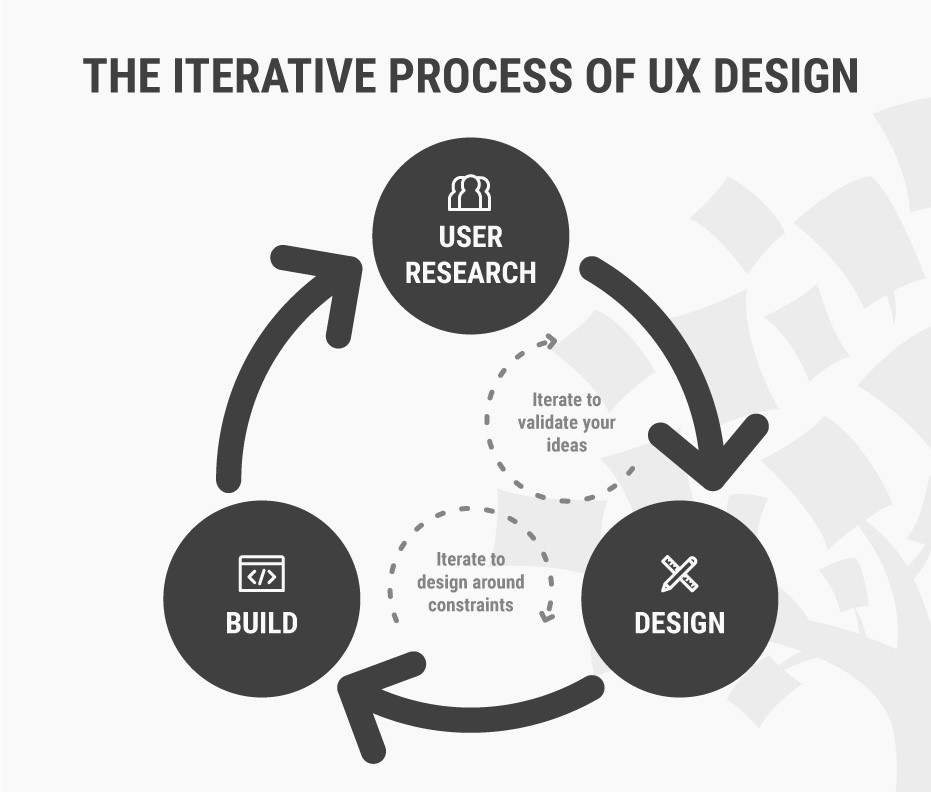
\includegraphics[width=\linewidth]{figures/ux-design}
	\caption{UX-Design.\cite{UXD}}
	\label{fig:ux-design}
\end{figure}


\section{Wireframe}

A wireframe is a methodology of showing a blueprint of a certain product. For example, if we consider to Wireframe a User Interface of an Application. It means to show a blueprint design of how the Application UI look like with different elements like buttons, text boxes etc placed on it and also how they interact and navigate to other User Interfaces. The blueprint design could vary from low fidelity i.e., rough sketches to high fidelity i.e., a more closer look to the desired final UI. There are several tools available in the market to do Wireframe and Balsamiq \cite{B} is one such tool. It is a kind of prototyping the actual product with certain simulation in functionality and visualization of the actual product. The advantage of this is the easiness of finding the mistakes in design earlier and so the cost of fixing them would be less. Here is an example of Website Wireframe is shown in the following figure \ref{fig:wireframe_website} of what one could design using Balsamiq tool and discuss with peers how they feel or to oneself to draw the ideas of what they want to achieve before actually coding to get the web page with the desired UI. \\ \\

\begin{figure}[hbt!]
	\centering
	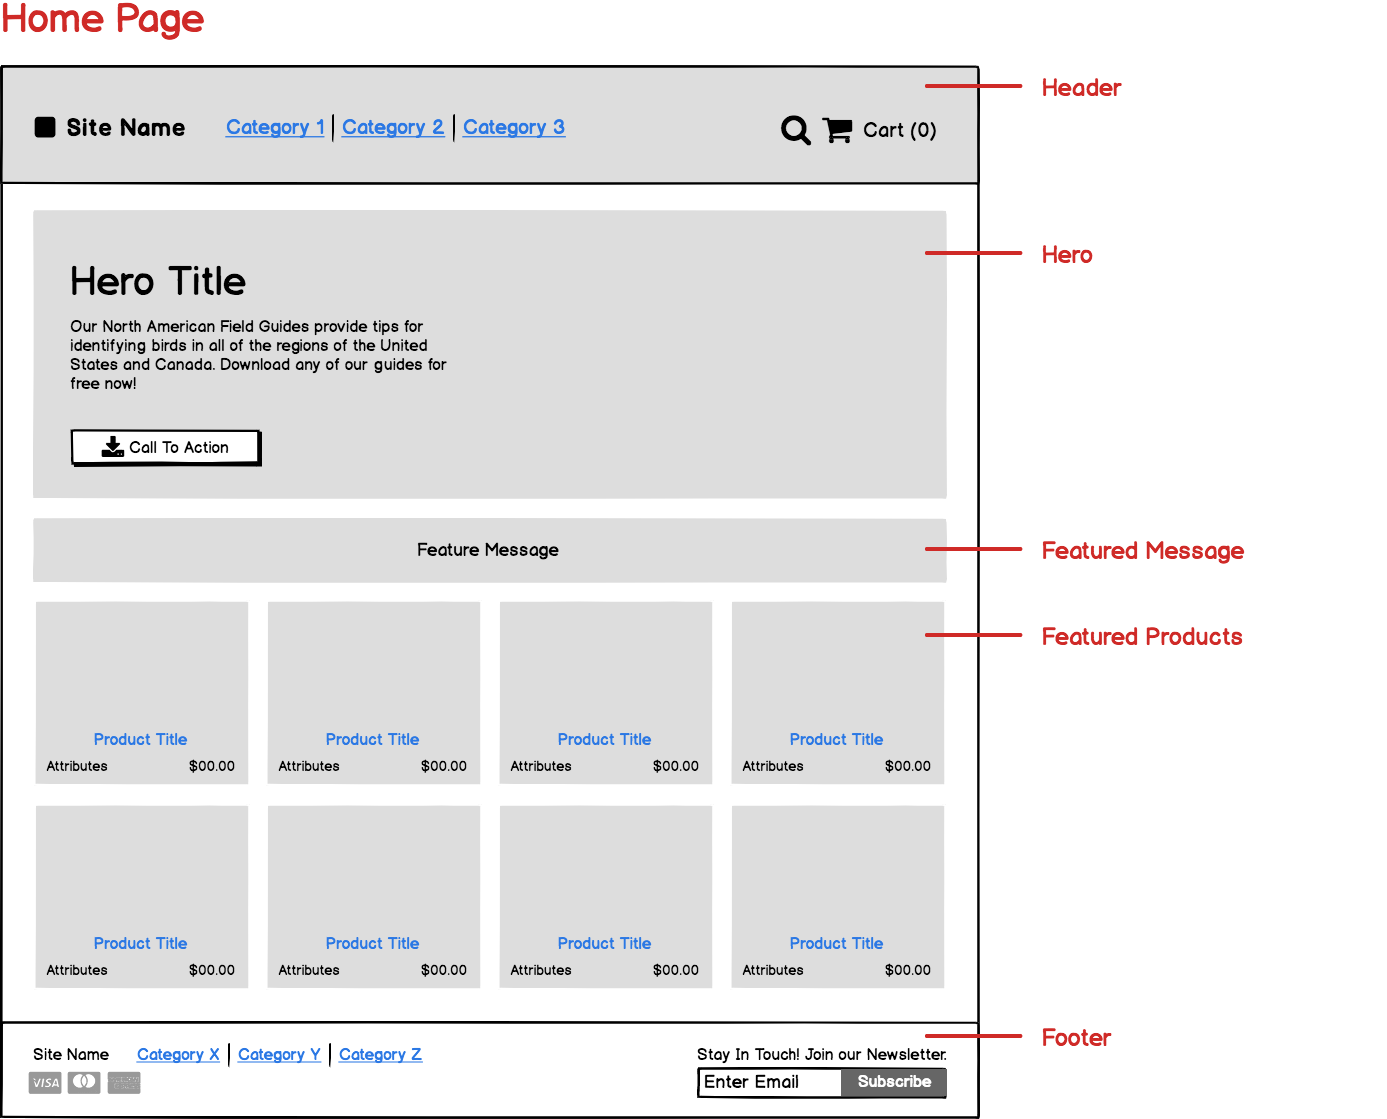
\includegraphics[width=\linewidth]{figures/wireframe_website}
	\caption{Website Wireframe.\cite{B}}
	\label{fig:wireframe_website}
\end{figure}

\let\cleardoublepage\clearpage
\chapter{Related Work}
\label{ch:relatedwork}

In order to tackle the research questions, different disciplines of software engineering such as Complex datasets, Compiler reporting, Continuous integration, Refactoring tools, Issue tracker, Stack Overflow, Gamification, Usability Engineering etc. are looked into and studied what ideas can be adapted into our scenario along with own novel solution ideas. \\ \\

After the literature review in above-mentioned disciplines, here are a few important takeaways in the scope of this Thesis. In the area of 'Complex datasets', current research where Dix et. al. \cite{Dix} talks about more complex grouping and linking of datasets in the context of a user interface of Spreadsheets application. There could be two datasets with fields having similar meaning and fields which are completely different. So, the key takeaway is about design lessons of extensibility of columns for example, 'venues were geocoded to allow spatial graphs' could be related as an example dates in bug reports to some standard format for all tools used and shown on a unified interface. Next, Gaur et. al. \cite{Gaur} speaks about the linear search problem in indexing as it takes more time for large volumes of data. So, different parameters are introduced to decrease computation time. Example: a database with toys is searched linearly for a given query it takes more time than a modified query let's say a toy in red colour and type horse then the search is simplified by looking at two parameters i.e, colour and type. This sparks the idea of grouping bugs as per module, bug type which could ease user in finding a certain bug on an interface.  \\ \\

In the area of 'Compiler reporting', Horning et. al. \cite{horning} mentions the importance of error logging with statistics as to what the compilers are expected to tell the user. It also mentions, the importance of stating what kind of bugs are not found along with bugs found but in reality this questions the scalability. So, the key takeaway is it is ideal to show the number of certain bugs founds in an analysis. Next in the area of 'Refactoring tools', Dustinca \cite{dustinca} talks about how the Refactoring tools are to be built and in user context, it has to overcome the barrier of discoverability which means the difficulty of use. To assist the developer on this issue, they introduced a smart tag in the context of user editor and notifies which parts of the code can be refactored. This emphasizes the importance of 'on-board' phase which plays a key role in Gamification \cite{gamify} discipline. Hayashi et. al. \cite{Hayashi} illustrates the importance of task level commits in order to maintain edit history of refactorings. This gives an idea of which a user does a bug-fix level commit to addressing the traceability scenario. Mealy et. al. \cite{Mealy} mentions about the importance of usability for software refactoring tools and this could perhaps give some basic guidelines similar to knowing Usability Engineering \cite{usability} discipline. \\ \\

In the area of 'Issue tracker', Baysal et. al. \cite{Baysal} mentions reducing the information overload for a developer in using the issue tracker. It is found out in their research paper that there is a too much of information they receive which in fact confuses the developer in how to react, example: the developer receive a high number of bugs reported via email and this leads to a situation where the developer ignore the email. They found out some interesting solution ideas such as having a private dashboard for each developer as it becomes easy to react to issues correspond to them. Expressiveness is one other mentioned in their paper which says an example, severity or priority are vague terms to describe a bug. Perhaps, it is ideal to describe the priory as per team decision instead of personal choice.  This signifies in categorising the results as per categories in our unified interface. Next in 'Stack Overflow', in a research paper by Wang et. al. \cite{stack} it is found there are 10934198 questions on a 'User Interface' topic for example. It is quite challenging to go through such a high volume database but nevertheless, the Stack Overflow team has a friendly user interface as shown in the following  \autoref{fig:stackoverflow}. It uses some clean filter techniques like tags for each topic, priority and trending etc. A research by Treude et. al. \cite{Treude.2011} found out that most of the questions (72.30\%) in Stack Overflow have between 2 and 4 tags. This could perhaps ease in filtering/indexing issues. \\ \\

\begin{figure}[hbt!]
	\centering
	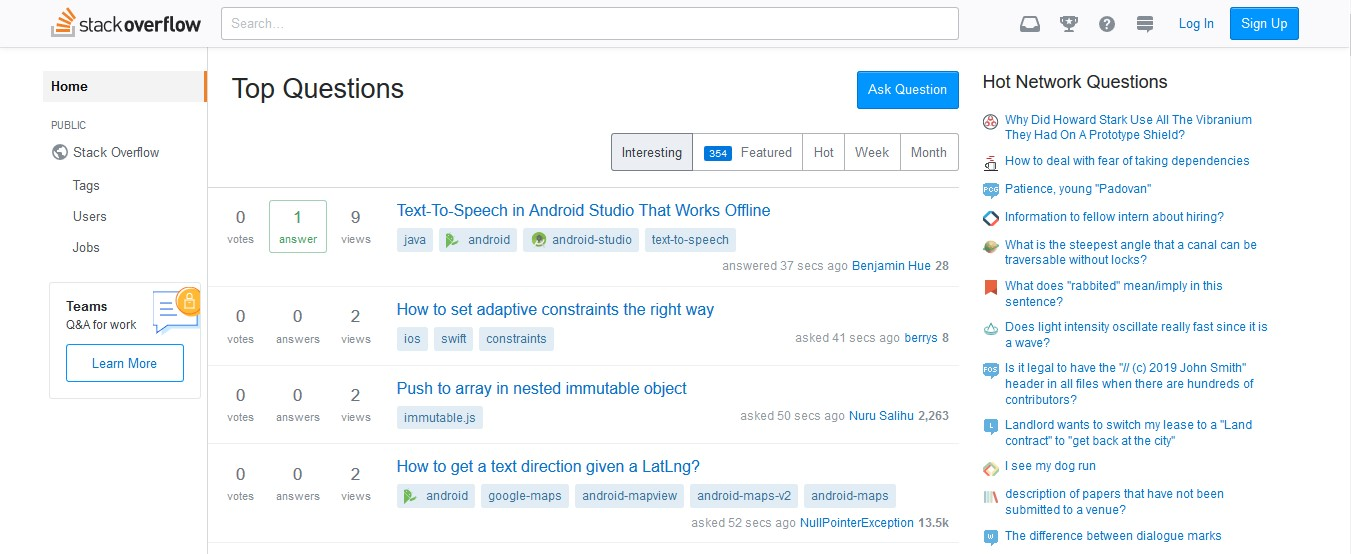
\includegraphics[width=\linewidth]{figures/stackoverflow}
	\caption{An user interface of Stack Overflow Website. \cite{stackoverflow}}
	\label{fig:stackoverflow}
\end{figure}
\chapter{Motivation}
\label{ch:motivation}

\section{Related Work}

Static Analysis plays a prominent role in releasing bug-free Software. In spite of that, important tools suffer from well-documented usability issues \cite{CB16,JSMB13}.  Maria et. al. \cite{CB16} did an empirical study on what developers want and need from Program Analysis. They noticed that there are some obstacles which hinder the usage of a Static Analysis tool by a developer such as 'Wrong checks are on by default', 'Too many false positives', 'Too slow',  'Complex user interface' etc. Being a user interface an obstacle for a developer is noteworthy. Johnson et. al. \cite{JSMB13} also found design flaws in current Static Analysis tools and the need for an interactive mechanism in assisting developers in fixing bugs. The interesting findings are like if the output of static analysis tool is user friendly and intuitive then false positives and high number of warnings could be less problematic for a developer, showing call hierarchies with which parts of code are affected by a bug, be able to share settings with predefined coding standards among the team, need of a web browser for reacting on the analysis output for instance adding comment to a bug which goes out of context to the developer. The key takes away from the above-mentioned papers is the importance of Usability in the ongoing adaption of Static Analysis tools. \\ \\ 

In general, the setup of most of the recent research \cite{CB16} \cite{JSMB13} done in the area of Static Code Analysis is like assuming a single project in an organisation. Further, they assume there is a single person working on a single project with a single tool tackling a single type of problems.  Somehow, the assumptions are made so singular to address a specific issue in their research. However, in practice i.e., in the real world of software engineering, there are numerous people working in teams for multiple projects at a time. Each project uses multiple tools in their software development. Even in the case of Static Code Analysis, multiple tools are used which are each capable of addressing several types of issues. \\ \\

\section{Current Research}

In the current research, we could see the usage of multiple tools in the Software Industry where each tool is different in computation approaches as one could be standard run on Nightly builds for example with Checkmarx \cite{checkmarx} tool or could be following Incremental Analysis, which means only testing the changed version of code instead of running analysis on complete codebase. The reasons of using multiple tools could be as each tool is capable of detecting bugs with different coverage \cite{bessey2010few} \cite{delaitre2015evaluating}, it could help in finding more bugs easily which are not found by tool but the other \cite{plakosh2014improving}. There is also research \cite{flynn2018prioritizing} going in the direction of using multiple static analysis tools in order to prioritise the bug warning alerts. There is a paper \cite{meng2008approach} published in 2008 which uses results of three different static analysis tools for a programming language, Java and merges them together in order to show warnings to the developer. Also, recently a team from OASIS \cite{oasis} in the OASIS SARIF Technical Committee \cite{oasis-tc} introduced a Static Analysis Results Interchange Format (SARIF) of representing bug warnings in a JSON format. Currently \cite{sarif-git}, the specification is being standardised. This shows there is potential research going in direction of using multiple static analysis tools at once. This shows the potential of using multiple tools in near future once the standardisation is adapted across static analysis tools developers or at least with the availability of adapters which are capable of converting the output of one static analysis tool to a SARIF format. Here's an example \cite{sarif-example} of how SARIF might look. SARIF is been used by SWAMP \cite{swamp-scarf-sarif}, a continuous software assurance which is automated.

\begin{lstlisting}[language=json,firstnumber=1][frame=single]

"results": [
{
"ruleId": "GSV001",
"message": {
"text": "Variable \"i\" was used without being initialized.",
"richText": "Variable `i` was used without being initialized." 
},
"locations": [
{
"physicalLocation": {
"uri": "file://build.example.com/work/src/collections/list.cpp", "region": {
"startLine": 16
}
},
"fullyQualifiedLogicalName": "collections::list:add"
}
]


\end{lstlisting}


Although we have seen the current research trends and their direction, the usability aspect is not addressed so far in the context of using multiple tools. The multiplicity of tools used for a single project and that too with different computation capabilities brings a new challenge.  One tool could produce results in no time and others could take more time in comparison. This could lead to a situation of breaking the usability of the user interface. On that challenge, this Thesis aims to address such a scenario with a problem statement as " How to integrate the results of multiple static analysis tools in a unified user interface? ".  \\ \\

The Thesis work begins by brainstorming on the problem statement and as a result, different research questions are brought up and of which three research questions are selected with respect to available sources, scope and limitations of Thesis time frame. \\ \\

\section{What current tools do?}

Let us now examine each research question and see what the current tools behave like. \\ \\

\textbf{1. How to display results for the same codebase from different analysis tools?}  \\

This question needs to address the scalability aspect of displaying results as usage of multiple tools results in redundancy and a high number of warnings with more coverage. The following figure \ref{fig:findbugs-results} shows how a FindBugs \cite{findbugs} static analysis tool shows results for a project \cite{findbugs-example}. This could be the same with other tool and so when you use multiple tools, there is a need for a better user interface.\\ \\

\begin{figure}[hbt!]
	\centering
	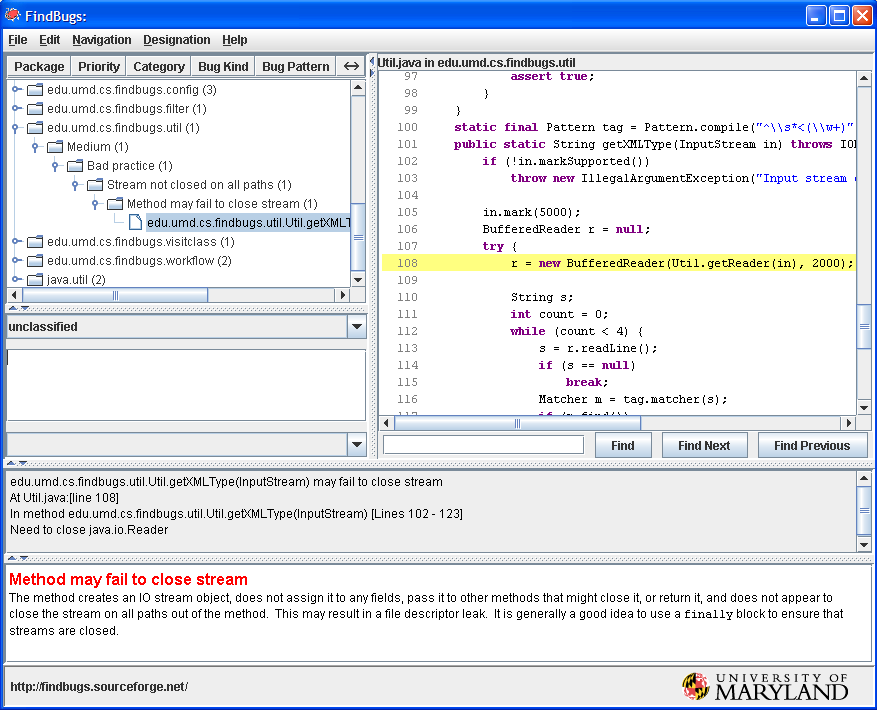
\includegraphics[width=\linewidth]{figures/findbugs-results}
	\caption{A preview of FindBugs scan results.}
	\label{fig:findbugs-results}
\end{figure}

\clearpage

\textbf{2. What feedback works to know that the bug fixing is on-going?} \\

This question needs to address the scenario where one tool could give an instant update on the bug fixing process and others might take more time to analyse and report the update on it. In the design aspect, especially the User Interface needs to be adaptive \cite{NB18} enough as static analysis tools sometimes take a long time to stop and there is no intuitive feedback provided. Also, One interesting aspect of Johnson et. al. \cite{JSMB13} study is about the importance of feedback from tools without disrupting the developer workflow. Traditionally, the project files are added to FindBugs \cite{findbugs} tool as seen in the figure \ref{fig:findbugs-scan} in order to start the scanning and the user has to wait for some minutes to see the results. There was no feedback in the process of scanning. \\ \\

\begin{figure}[hbt!]
	\centering
	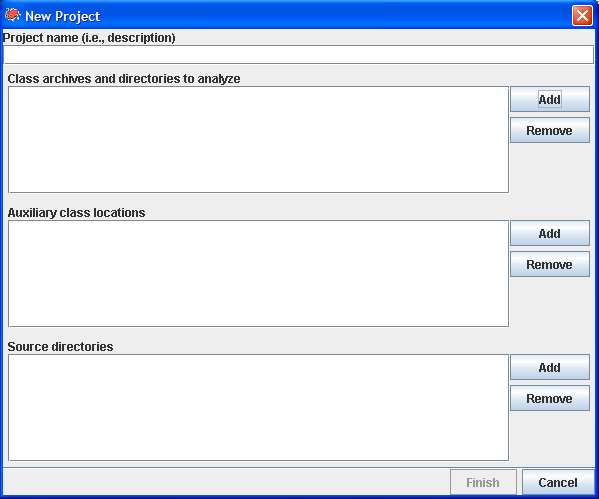
\includegraphics[width=\linewidth]{figures/findbugs-scan}
	\caption{A preview of initiating FindBugs to scan a project.}
	\label{fig:findbugs-scan}
\end{figure}

Back in the history of Computer Science, there is an observation made when the user interface is non-responsive, the user shuts down the system. Thereafter, comes to the implementation of user interface called Ghost screen by Colleran et al. \cite{colleran} who patented the method which manages application programs with non-responsive user interfaces in the year 2005. About the response times, NN Group \cite{nn} states that if the execution of a certain task takes 0.1 up to 1 second then there is no need for feedback, just show the result. If it takes 10 seconds, there should be feedback and if it is variable every time then there is the importance of per cent bar \cite{Borman} but sometimes it could be overkill to use as it cause stress to the user by the principle of display inertia. If the time taken by a task is unknown then there has to be feedback like a spinning ball or in an example of a task being to scan databases then it has to report user what database is being scanned currently. Overall, there has to be feedback stating that the system is working, if not indicating what is actually doing. This motivates to know how responsiveness in terms of usability is vital to consider in the development of modern tools. Further, this needs to be addressed in the context of using multiple tools.\\ \\


\textbf{3. How to carry traceability of bug fixing?} \\

In the scenario, where the user has picked a bug to fix and worked on it and later he submitted for analysis. Then the bug could either get fixed or new bugs could have been introduced or different bugs got resolved by fixing the one bug. All these might have taken place and this is uncertain. Thereby it would be better to have traceability in order to somehow safeguard the code repository from future bugs or monitor the changes happening in the context of bugs. \\ \\

As per the related work in research \cite{heinemann2014teamscale}, a tool named "Teamscale" \cite{teamscale} shows the influence on the quality status for each change in code backed by version control commits. For a change, it shows how many quality problems are added or removed. The illustration could be observed in the following figure \ref{fig:teamscale}.\\ \\

\begin{figure}[hbt!]
	\centering
	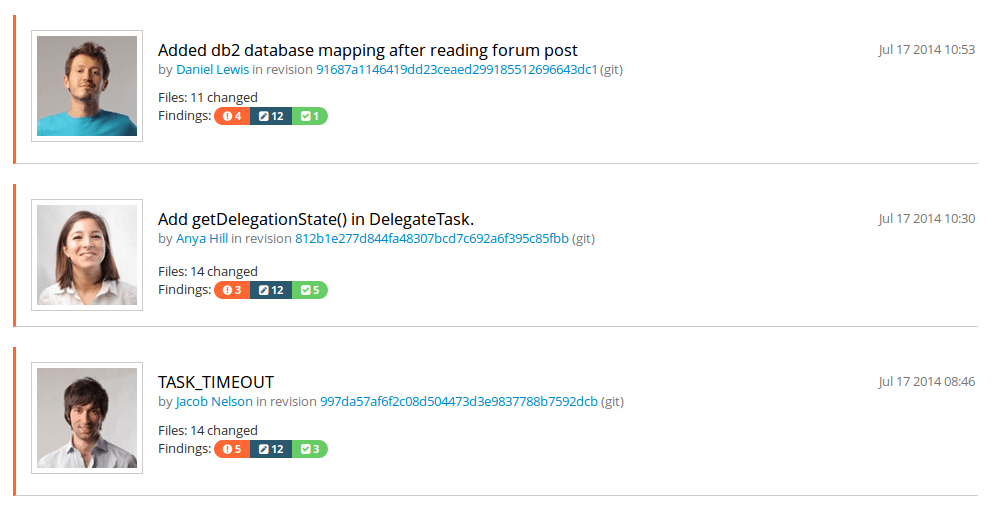
\includegraphics[width=\linewidth]{figures/teamscale}
	\caption{A Teamscale feature of showing quality status with code changes.}
	\label{fig:teamscale}
\end{figure}

\let\cleardoublepage\clearpage

\chapter{Objectives}
\label{ch:objectives}

Static analysis tools suffer from well-documented usability issues \cite{CB16,JSMB13}. In the current research, it is found out that a typical software organisation uses multiple static analysis tools. This leads to the issue where the user interface has to be adaptive in integrating such different tools. \\ \\ \\
In this thesis, it is researched on different user interface designs that allow code developers to navigate around
this issue in a non-disruptive way. \\ \\ \\
1. Research different techniques as mentioned in \autoref{ch:approaches} that tackle the respective research question in other domains of software
engineering. \\ \\
2. Adapt those techniques and design prototypes with own techniques for the domain of static analysis. \\ \\
3. Design prototypes with a Balsamiq wireframe tool \cite{B} of those techniques to improve the usability of integrating analysis tools. \\ \\
4. Design user studies that evaluate the efficiency of those techniques, with professional code developers. \\ \\
5. Run the user studies and report on their results. \\ \\
6. Loop 2 $\rightarrow$ 5 until desired outcome towards good user experience is achieved.

\let\cleardoublepage\clearpage
\chapter{Approaches}
\label{ch:approaches}

\chapter{Evaluation Plan}
\label{ch:evaluationplan} 

The prototypes designed with approaches mentioned in the earlier chapter are evaluated as per the below experiment design guidelines. \\ \\

\section{Experiment Design}

\subsection{Number of Test Users}

The target users for evaluation are experienced software developers who have good knowledge of software development in general and used one of static analysis tool in their development process. So, if not the professional software developers at least the students pursuing a Masters degree in Computer Science. This ensures the evaluation process to be valid and authentic. There will be five users selected for evaluating the prototypes. One might be surprised about why only five users required, the reason behind that is well explained by Human-Computer Interaction researcher Mr. Jakob Nielsen with a simple formula\cite{five}. \\ \\

\[ N (1-(1- L )^n ) \]

Where \textbf{N} is the total number of usability problems exist in the given design, \textbf{L} is the proportion of usability problems discovered while testing a single user which is typically 31\% as found in his research. The below plot \ref{fig:5plot} further illustrates that after the number of users is five then the usability problems discovered does not increase much further as there would be high overlap with already found usability problems by previous users. Thereby, five users are selected for each iteration of the User Experience Design cycle to test the prototype designs. \\ \\

\begin{figure}[hbt!]
	\centering
	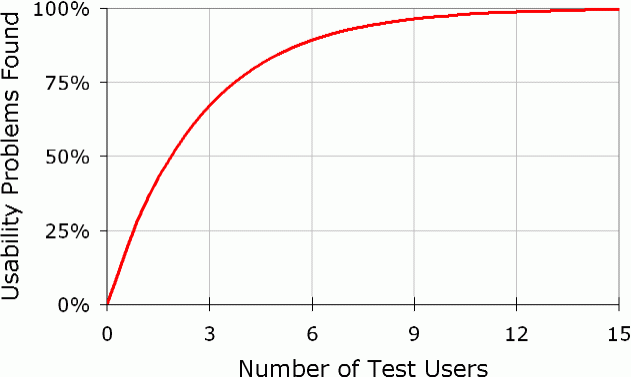
\includegraphics[width=\linewidth]{figures/fiveplot}
	\caption{A plot illustrating the usability problems found with the users.}
	\label{fig:5plot}
\end{figure}

\subsection{Order of Evaluation}

As the order of prototypes with different solution ideas presented in evaluation could influence the user as they tend to learn. Therefore, the order is changed for different segments of users which could lead to a qualitative result. For instance, let us say there are two prototypes named A and B. Half of users i..e, three in our case will have prototype A evaluated first and another half i.e., two users will evaluate B first. \\ \\

\section{Usability Inspection Methods}

There are many Usability inspection methods \cite{nielsen1994usability} like Heuristic evaluation, Heuristic estimation, Cognitive walkthrough, Pluralistic walkthrough, Feature inspection, Consistency inspection, Standards inspection and Formal usability inspection.  Out of which, the Usability aspect of the prototypes are evaluated with  'Cognitive walkthrough' and 'Heuristic evaluation'. \\ \\

\subsection{Cognitive Walkthrough}

In Cognitive walkthrough, users are asked to perform tasks with predefined steps. For each step, there are questions examined to determine usability. Blackmon, Polson, et al. in their paper \cite{blackmon2002cognitive} mentions four questions which are significant to analyse while performing Cognitive Walkthrough for the Web. They are;  \\ \\

\begin{enumerate}
	\item Will the user try and achieve the right outcome?	
	\item Will the user notice that the correct action is available to them?
	\item Will the user associate the correct action with the outcome they expect to achieve?
	\item If the correct action is performed; will the user see that progress is being made towards their intended outcome?
\end{enumerate}

These questions are also quite applicable in our context. Thereby, these questions are assessed for each step which is predetermined with designed elements on the user interface in order to solve the Research question been tackled. So, the steps vary for each design. This approach gives qualitative feedback from a user as they are a mostly open-ended scenario to discuss especially, for questions which are answered as 'No' would lead to having their suggestions/feedback. \\ \\

\subsection{Heuristic Evaluation}

In a Heuristic evaluation, the overall design is evaluated after the user has gone through the interface once or twice understanding the workflow/architecture. Then the design is evaluated with Heuristics which are called rules of thumb in the examination of usability problems. Nielsen proposed ten heuristics as standard such as, Visibility of system status, Match between system and the real world, User control and freedom, Consistency and standards, Error prevention, Recognition rather than recall, Flexibility and efficiency of use, Aesthetic and minimalist design, Help users recognize, diagnose, and recover from errors and Help and documentation. \\ \\

Once the evaluator went through the design twice, he/she mentions the problems in the context of certain heuristic. They could go through each problem mentioned with severity rating ranging from 0 to 4, where 0 - do not agree this is a usability problem, 1 - cosmetic problem, 2 - minor usability problem, 3 - major usability problem ( important to fix ), 4 - usability catastrophe ( imperative to fix ). Finally, the list of problems with severity is gathered from all evaluators. Then, the accumulated results help in re-designing the prototypes taking care that the current issues are addressed for the next iteration of the User Experience Design cycle. This evaluation process also gives valuable qualitative feedback. \\ \\

Overall, both Cognitive walkthrough and Heuristic evaluation helps to identify the usability problems in detail as possible which is qualitative analysis. Further, when more than two best solution ideas are needed to evaluated against each other then a Heuristic estimate method could be considered. It is simply to estimate which is more accepted by users with a parameter of the majority, where more number of users/evaluators could determine the stronger validity of voting which is quantitative analysis. \\ \\

\let\cleardoublepage\clearpage
\chapter{Time Plan}
\label{ch:timeplan}

The Thesis work assumed to follow the below time plan as shown in \autoref{fig:time-plan} as a standard framework. It is primarily focussed on three iterations of the UX Design process with a proper user study as a minimum with the limitation of Thesis time i.e., five months. However, with available resources will strive to perform possible UX Design cycle iterations and reach quality output with this Thesis work. \\

Each UX Design cycle iteration is planned for one month. It comprises of four steps such as, developing prototypes, plan user study, hold user study and finally assimilating the results of that iteration. Each step is planned to execute in a week time. Next, after an iteration, again develop prototypes with improvements based on previous iteration results. Thereby, three iterations are planned as seen in  \autoref{fig:time-plan}. \\ 

\textbf{Milestone 1} \\

As the first milestone, by the end of May month, the first iteration of the UX Design Cycle has to be completed. \\ 

\textbf{Milestone 2} \\

As the second milestone, by the end of June month, the second iteration of the UX Design Cycle has to be completed. \\ 

\textbf{Milestone 3} \\

As the third milestone, by the end of July month, the third iteration of yhe UX Design Cycle has to be completed. \\

\textbf{Milestone 4} \\

As the fourth and the final milestone, by the end of September month, the Thesis documentation including presentation has to be completed. \\

 
\begin{figure}
	\centering
	\scalebox{0.8}{	\begin{tikzpicture}
		\begin{pgfinterruptboundingbox}
		\begin{ganttchart}[Mile/.style={milestone/.append style={fill=red,xscale=5}}, canvas/.append style={alias=frame}, title/.style={fill=blue, draw=none},
		title label font=\color{white}\bfseries,
		time slot format=isodate,
		title right shift=-.1,
		title top shift=.05,
		x unit=1mm
		]{2019-06-01}{2019-10-30}		
		\gantttitlecalendar{year,month=name} \\   	
		
		\ganttgroup[group/.append style={draw=black, fill=teal!50}]{UX Design Cycle 1}{2019-06-01}{2019-06-30} \\	
		\ganttbar[bar/.append style={fill=green!50}]{Develop Prototypes}{2019-06-01}{2019-06-07} \\
		\ganttbar[bar/.append style={fill=green!50}]{Plan User Study}{2019-06-08}{2019-06-14} \\
		\ganttbar[bar/.append style={fill=green!50}]{Hold User Study}{2019-06-15}{2019-06-21} \\
		\ganttbar[bar/.append style={fill=green!50}]{Assimilate Results}{2019-06-22}{2019-06-30} \\
		\ganttmilestone[Mile]{Milestone 2}{2019-06-30} \\
		
		\ganttgroup[group/.append style={draw=black, fill=teal!50}]{UX Design Cycle 2}{2019-07-01}{2019-07-31} \\	
		\ganttbar[bar/.append style={fill=green!50}]{Develop Prototypes}{2019-07-01}{2019-07-07} \\
		\ganttbar[bar/.append style={fill=green!50}]{Plan User Study}{2019-07-08}{2019-07-14} \\
		\ganttbar[bar/.append style={fill=green!50}]{Hold User Study}{2019-07-15}{2019-07-21} \\
		\ganttbar[bar/.append style={fill=green!50}]{Assimilate Results}{2019-07-22}{2019-07-31} \\
		\ganttmilestone[Mile]{Milestone 3}{2019-07-31} \\
		
		\ganttgroup[group/.append style={draw=black, fill=teal!50}]{UX Design Cycle 1}{2019-08-01}{2019-08-31} \\	
		\ganttbar[bar/.append style={fill=green!50}]{Develop Prototypes}{2019-08-01}{2019-08-07} \\
		\ganttbar[bar/.append style={fill=green!50}]{Plan User Study}{2019-08-08}{2019-08-14} \\
		\ganttbar[bar/.append style={fill=green!50}]{Hold User Study}{2019-08-15}{2019-08-21} \\
		\ganttbar[bar/.append style={fill=green!50}]{Assimilate Results}{2019-08-22}{2019-08-31} \\
		\ganttmilestone[Mile]{Milestone 1}{2019-08-31} \\
		
		\ganttgroup[group/.append style={draw=black, fill=teal!50}]{Documentation Phase }{2019-09-01}{2019-10-30} \\	
		\ganttbar[bar/.append style={fill=green!50}]{Documenatation}{2019-09-01}{2019-10-30} \\
		\ganttbar[bar/.append style={fill=green!50}]{Presentation}{2019-09-25}{2019-10-30} \\
		\ganttbar[bar/.append style={fill=green!50}]{Review}{2019-10-01}{2019-10-30} \\
		\ganttmilestone[Mile]{Milestone 4}{2019-10-28}
		
		\end{ganttchart}	
		\end{pgfinterruptboundingbox}
		\useasboundingbox (frame.south west) rectangle (frame.north east);
		\end{tikzpicture} }
	\caption{Thesis Official Time Plan}	
	\label{fig:time-plan}
\end{figure}


\chapter{Conclusion}
\label{ch:conclusion}


As software became a part of a day to day life, bug-free software is quite necessary. For which, static code analysis tools are used to identify and mitigate bugs during software development life cycle. Although there are essential tools, in terms of usability they lack to have the attention of developers. Further, the use of multiple static code analysis tools is increasing for obvious reasons like to ensure the bug priority, increase coverage area etc. On the other hand, there is a standardisation process going on with SARIF format and this promises to have generated results in the same format from different analysis tools. \\ \\

Thereby, this shows the future scope of ongoing research with multiple tools usage. So, when the integration of results from different tools happens, it is necessary to be usable for better usage by developers. This thesis aims to address this issue with three different research questions i.e., \\ 1. How to display results of the same codebase from different analysis tools? \\
2. What feedback works to know that the bug fixing is on-going? \\
3. How to carry traceability of bug fixing? \\ \\

The research questions are answered by studying different software engineering disciplines and adapt the possible techniques if any. Also, the developers' feedback is analysed through user experience design cycle to make sure the designed prototypes are usable enough to overcome the issues. Hence, the thesis work ensures the applicability of results examined.

% include the bibliography, and add it as a chapter the table of contents
\newpage
\addcontentsline{toc}{chapter}{Bibliography}
\printbibliography 


%%%%%%%%%
% the appendices of your thesis go into file appendix.tex
%%%%%%%%%
\appendix
\chapter{List of Abbrevations}

\textbf{UI} - User Interface \\ \\
\textbf{UX} - User Experience \\ \\
\textbf{CLI} - Command Line Interface \\ \\
\textbf{GUI} - Graphical User Interface \\ \\
\textbf{MSAT-UI} - Multiple Static Analysis Tools User Interface \\ \\

\end{document}
